% Ringkasan 20 slide. Kompilasi: pdfLaTeX dua kali.
% Acuan: silabus minggu 1--7 dan ETS_FISMAT_I-2.pdf.
% Mandiri: tanpa berkas input atau gambar eksternal.
\documentclass[11pt,aspectratio=169]{beamer}
\usepackage[T1]{fontenc}
\usepackage[utf8]{inputenc}
\usepackage{lmodern}
\usepackage{amsmath,amssymb,mathtools,booktabs,array}
\usepackage{tikz}
\usetikzlibrary{arrows.meta,calc}
% Latar hangat, teks arang, dan satu aksen biru keabu-abuan.
\definecolor{Paper}{HTML}{F8F7F4}
\definecolor{Ink}{HTML}{293239}
\definecolor{Accent}{HTML}{536B75}
\definecolor{Muted}{HTML}{626B70}
\definecolor{Rule}{HTML}{D7DAD8}
\setbeamercolor{normal text}{fg=Ink,bg=Paper}
\setbeamercolor{structure}{fg=Accent}
\setbeamercolor{frametitle}{fg=Ink,bg=Paper}
\setbeamercolor{title}{fg=Ink}
\setbeamercolor{block title}{fg=Accent,bg=Paper}
\setbeamercolor{block body}{fg=Ink,bg=Paper}
\setbeamercolor{footline}{fg=Muted,bg=Paper}
\setbeamerfont{frametitle}{size=\large,series=\bfseries}
\setbeamerfont{block title}{size=\normalsize,series=\bfseries}
\setbeamerfont{footline}{size=\tiny}
\setbeamertemplate{navigation symbols}{}
\setbeamertemplate{blocks}[default]
\setbeamertemplate{itemize item}{\tiny\raisebox{.3ex}{\textbullet}}
\setbeamersize{text margin left=9mm,text margin right=9mm}
\setbeamertemplate{frametitle}{%
  \vspace{3mm}\insertframetitle\par\vspace{1.5mm}%
  {\color{Rule}\hrule height .4pt}\vspace{1mm}}
\setbeamertemplate{footline}{%
  \hbox{\begin{beamercolorbox}[wd=.84\paperwidth,ht=2.5ex,dp=1.5ex,leftskip=9mm]{footline}%
    FISIKA MATEMATIKA 1\quad /\quad RINGKASAN ETS
  \end{beamercolorbox}%
  \begin{beamercolorbox}[wd=.16\paperwidth,ht=2.5ex,dp=1.5ex,rightskip=9mm]{footline}%
    \hfill\insertframenumber\,/\,\inserttotalframenumber
  \end{beamercolorbox}}}
\setlength{\emergencystretch}{1.5em}
\newcommand{\vect}[1]{\boldsymbol{#1}}
\newcommand{\R}{\mathbb{R}}
\DeclareMathOperator{\Span}{span}
\DeclareMathOperator{\rank}{rank}
\DeclareMathOperator{\proj}{proj}
\DeclareMathOperator{\adj}{adj}
\title{Ringkasan Materi ETS}
\author{}
\date{}
\begin{document}

% 01
\begin{frame}[plain]
\vspace{8mm}
{\small\color{Accent}FISIKA MATEMATIKA 1}\par\vspace{4mm}
{\LARGE\bfseries Ringkasan Materi ETS}\par\vspace{3mm}
{\large Vektor, geometri, dan aljabar linier}\par\vspace{6mm}
{\color{Rule}\hrule height .5pt}\vspace{5mm}
\textbf{Gagasan penghubung}\par\smallskip
Vektor menyatakan besaran dan arah. Dot serta cross product membaca
geometrinya. Matriks menyatakan transformasi dan sistem persamaan.
\vfill
{\footnotesize\color{Muted}Cakupan minggu 1--7\enspace\textbullet\enspace
Konsep, makna fisika, dan penurunan rumus singkat}
\end{frame}

\section{Vektor dan makna fisikanya}

% 02
\begin{frame}{Vektor: objeknya tetap, komponennya bergantung pada basis}
Basis Kartesius ortonormal $\mathbf{i},\mathbf{j},\mathbf{k}$ searah sumbu $x,y,z$:
\[
\vect{a}=a_x\mathbf{i}+a_y\mathbf{j}+a_z\mathbf{k},
\qquad \|\vect{a}\|=\sqrt{a_x^2+a_y^2+a_z^2}.
\]
\begin{itemize}
\item Penjumlahan vektor dan perkalian skalar dilakukan per komponen.
\item Vektor satuan $\widehat{\vect{a}}=\vect{a}/\|\vect{a}\|$ memisahkan
\textbf{arah} dari \textbf{besar}, untuk $\vect{a}\ne\vect{0}$.
\item Perpindahan, kecepatan, dan gaya adalah contoh vektor.
Mengubah sumbu koordinat tidak mengubah besaran fisiknya.
\end{itemize}
\begin{block}{Contoh singkat}
$\vect{a}=(2,-1,2)$ memiliki besar $3$.
Vektor searah dengan besar $12$ ialah $12\widehat{\vect{a}}=(8,-4,8)$.
\end{block}
\end{frame}

% 03
\begin{frame}{Dot product mengukur seberapa searah dua vektor}
\[
\boxed{\vect{a}\cdot\vect{b}=\sum_i a_i b_i
=\|\vect{a}\|\,\|\vect{b}\|\cos\theta}
\]
\small
\renewcommand{\arraystretch}{1.25}
\begin{tabular}{@{}>{\raggedright\arraybackslash}p{.22\textwidth}>{\raggedright\arraybackslash}p{.32\textwidth}>{\raggedright\arraybackslash}p{.39\textwidth}@{}}
\toprule
\textbf{Besaran fisika} & \textbf{Hubungan} & \textbf{Makna}\\
\midrule
Usaha gaya konstan & $W=\vect{F}\cdot\Delta\vect{r}$ & Hanya komponen gaya searah perpindahan yang melakukan usaha.\\
Daya sesaat & $P=\vect{F}\cdot\vect{v}$ & Laju usaha bergantung pada arah kecepatan.\\
Fluks medan listrik & $\Phi_E=\int_S\vect{E}\cdot\widehat{\vect{n}}\,dA$ & Komponen medan yang menembus permukaan yang dihitung.\\
\bottomrule
\end{tabular}
\medskip
\textbf{Fakta:} gaya tegak lurus perpindahan menghasilkan usaha nol,
walaupun gayanya tidak nol. Untuk vektor tak nol, dot positif pada sudut lancip dan negatif pada sudut tumpul.
\end{frame}

% 04
\begin{frame}{Proyeksi: asal rumus dan komponen gaya}
Tuliskan komponen $\vect{a}$ sepanjang $\vect{b}\ne\vect{0}$ sebagai
$\vect{a}_{\parallel}=\alpha\vect{b}$. Sisanya harus tegak lurus $\vect{b}$:
\[
(\vect{a}-\alpha\vect{b})\cdot\vect{b}=0
\quad\Longrightarrow\quad
\boxed{\proj_{\vect{b}}\vect{a}
=\frac{\vect{a}\cdot\vect{b}}{\|\vect{b}\|^2}\vect{b}}.
\]
\[
\vect{a}_{\perp}=\vect{a}-\vect{a}_{\parallel},\qquad
\|\vect{a}\|^2=\|\vect{a}_{\parallel}\|^2+\|\vect{a}_{\perp}\|^2.
\]
\begin{block}{Mengapa muncul $F\cos\theta$?}
Komponen skalar gaya pada arah satuan $\widehat{\vect{d}}$ ialah
$F_{\parallel}=\vect{F}\cdot\widehat{\vect{d}}=F\cos\theta$.
Komponen ini bertanda; panjang proyeksi adalah $|F_{\parallel}|$.
\end{block}
\end{frame}

% 05
\begin{frame}{Cross product membaca normal dan efek putaran}
\[
\vect{a}\times\vect{b}
=\begin{vmatrix}\mathbf{i}&\mathbf{j}&\mathbf{k}\\a_x&a_y&a_z\\b_x&b_y&b_z\end{vmatrix},
\qquad
\|\vect{a}\times\vect{b}\|=\|\vect{a}\|\,\|\vect{b}\|\sin\theta.
\]
\small
\begin{itemize}
\item Hasilnya \textbf{vektor normal} terhadap kedua faktor; arah mengikuti
kaidah tangan kanan. Urutan dibalik, tanda berubah.
\item \textbf{Torsi:} $\vect{\tau}=\vect{r}\times\vect{F}$.
Besar torsi $=F(r\sin\theta)$: gaya dikali lengan momen tegak lurus.
\item \textbf{Momentum sudut:} $\vect{L}=\vect{r}\times\vect{p}$,
diukur terhadap titik acuan yang dipilih.
\item \textbf{Gaya magnet:} $\vect{F}_B=q\vect{v}\times\vect{B}$.
Karena $\vect{F}_B\cdot\vect{v}=0$, gaya magnet tidak melakukan usaha pada partikel.
\end{itemize}
\textcolor{Accent}{Dot menghasilkan skalar; cross dalam $\R^3$ menghasilkan vektor.}
\end{frame}

% 06
\begin{frame}{Luas dan volume: dot dan cross saling terhubung}
\small
Untuk dua sisi segitiga $\vect{u},\vect{v}$ yang berpangkal sama,
\[
L_\triangle=\tfrac12\|\vect{u}\times\vect{v}\|
=\tfrac12\sqrt{\|\vect{u}\|^2\|\vect{v}\|^2-(\vect{u}\cdot\vect{v})^2}.
\]
\textbf{Bukti singkat:} kuadratkan rumus besar cross product,
lalu gunakan $\sin^2\theta=1-\cos^2\theta$ dan
$\vect{u}\cdot\vect{v}=\|\vect{u}\|\,\|\vect{v}\|\cos\theta$.
\begin{block}{Contoh dari PDF}
$P_1=(2,2,0)$, $P_2=(-1,0,2)$, $P_3=(0,4,3)$ memberi
$\vect{u}=(-3,-2,2)$, $\vect{v}=(-2,2,3)$.
\[
\vect{u}\times\vect{v}=(-10,5,-10),\qquad
L_\triangle=\tfrac{15}{2}=\tfrac12\sqrt{17\cdot17-8^2}.
\]
\end{block}
\textbf{Volume paralelipiped:} $V=|\vect{w}\cdot(\vect{u}\times\vect{v})|$.
Nilainya nol jika ketiga vektor koplanar.
\end{frame}

% 07
\begin{frame}{Span, bebas linier, dan basis}
\small
\begin{itemize}
\item \textbf{Span}: seluruh kombinasi $c_1\vect{v}_1+\cdots+c_k\vect{v}_k$.
\item \textbf{Bebas linier}: $\sum_i c_i\vect{v}_i=\vect{0}$ hanya jika seluruh $c_i=0$.
\item \textbf{Basis}: bebas linier dan membentang ruang;
jumlah anggotanya adalah dimensi ruang tersebut.
\end{itemize}
\[
W=\{(x,y,z):z=x+y\}
=\Span\{(1,0,1),(0,1,1)\},\qquad \dim W=2.
\]
Vektor $(1,1,2)$ adalah jumlah kedua vektor basis, sehingga menambahkannya
tidak menambah dimensi.
\begin{block}{Fakta penting untuk komponen fisika}
Koordinat pada basis selalu unik. Namun rumus $c_i=\vect{v}\cdot\vect{e}_i$
berlaku langsung hanya untuk \textbf{basis ortonormal}.
Pada basis umum, cari $c_i$ dari $\vect{v}=\sum_i c_i\vect{b}_i$.
\end{block}
\end{frame}

\section{Geometri dengan vektor}

% 08
\begin{frame}{Garis memakai arah; bidang memakai normal}
\begin{columns}[T,onlytextwidth]
\column{.48\textwidth}
\begin{block}{Garis}
Titik acuan $A$, arah $\vect{d}\ne\vect{0}$:
\[
\vect{r}=\vect{a}+t\vect{d},\quad t\in\R.
\]
Jika melalui $A$ dan $B$, pilih $\vect{d}=B-A$.
\end{block}
\column{.49\textwidth}
\begin{block}{Bidang}
Titik acuan $A$, normal $\vect{n}\ne\vect{0}$:
\[
\vect{n}\cdot(\vect{r}-\vect{a})=0.
\]
Jika melalui tiga titik tidak segaris,
\[
\vect{n}=(B-A)\times(C-A).
\]
\end{block}
\end{columns}
\medskip\small
\textbf{Fakta geometri:} garis tegak lurus bidang memiliki arah sejajar
$\vect{n}$. Jika $\vect{n}\cdot\vect{d}=0$, garis sejajar bidang atau terletak di dalamnya.
\medskip

Untuk $\vect{n}=(a,b,c)$, bentuk bidang adalah $ax+by+cz=d_0$.
Mengalikan seluruh persamaan dengan skalar tak nol tidak mengubah bidang.
\end{frame}

% 09
\begin{frame}{Dari cross product ke jarak titik--bidang}
\small
Ambil $A,B,C$ pada bidang, tidak segaris, dan titik $P$:
\[
\vect{u}=B-A,\quad\vect{v}=C-A,\quad\vect{w}=P-A,\quad
\vect{n}=\vect{u}\times\vect{v}.
\]
\begin{columns}[T,onlytextwidth]
\column{.64\textwidth}
Luas alas jajargenjang $S=\|\vect{u}\times\vect{v}\|$.
Volume sama dengan alas dikali tinggi:
\[
Sh=|\vect{w}\cdot(\vect{u}\times\vect{v})|,
\qquad h=\frac{|\vect{w}\cdot\vect{n}|}{\|\vect{n}\|}.
\]
Untuk $\vect{n}=(a,b,c)$ dan bidang $ax+by+cz=d_0$,
\[
\boxed{h=\frac{|ax_P+by_P+cz_P-d_0|}{\sqrt{a^2+b^2+c^2}}}.
\]
\column{.32\textwidth}
\centering
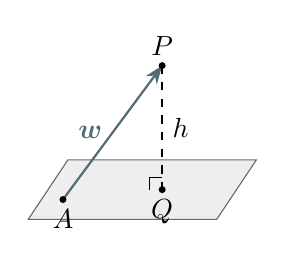
\begin{tikzpicture}[scale=.63,>=Stealth]
\filldraw[fill=Rule!45,draw=Muted] (0,0)--(3.8,0)--(4.6,1.2)--(.8,1.2)--cycle;
\coordinate (A) at (.7,.4); \coordinate (Q) at (2.7,.6); \coordinate (P) at (2.7,3.1);
\draw[->,thick,Accent] (A)--(P) node[midway,left] {$\vect{w}$};
\draw[dashed,thick] (P)--(Q) node[midway,right] {$h$};
\draw (2.45,.6)--(2.45,.85)--(2.7,.85);
\fill (A) circle(2pt) node[below] {$A$};
\fill (Q) circle(2pt) node[below] {$Q$};
\fill (P) circle(2pt) node[above] {$P$};
\end{tikzpicture}\par
\end{columns}
\medskip
\textcolor{Accent}{Cross membentuk normal dan luas alas; dot mengambil tinggi pada arah normal.}
\end{frame}

% 10
\begin{frame}{Titik terdekat adalah kaki proyeksi tegak lurus}
\small
Untuk bidang $\vect{n}\cdot\vect{r}=d_0$, tulis $\vect{q}=\vect{p}-\lambda\vect{n}$.
Syarat $Q$ berada di bidang memberi
\[
\vect{n}\cdot\vect{p}-\lambda\|\vect{n}\|^2=d_0
\quad\Longrightarrow\quad
\boxed{\vect{q}=\vect{p}-\frac{\vect{n}\cdot\vect{p}-d_0}{\|\vect{n}\|^2}\vect{n}}.
\]
\begin{block}{Contoh: $P=(3,2,3)$ dan bidang $2x+y+2z=2$}
\[
\vect{n}=(2,1,2),\qquad h=\frac{|6+2+6-2|}{3}=4,
\]
\[
Q=(3,2,3)-\frac{12}{9}(2,1,2)
=\left(\frac13,\frac23,\frac13\right).
\]
\end{block}
Jarak memakai nilai mutlak; rumus $Q$ mempertahankan tanda.
Cek: $Q$ memenuhi bidang dan $P-Q$ sejajar normal.
\end{frame}

% 11
\begin{frame}{Jarak titik--garis juga berasal dari luas}
\small
Garis $\ell:\vect{r}=\vect{a}+t\vect{d}$ dengan $\vect{d}\ne\vect{0}$.
Ambil $\vect{w}=\vect{p}-\vect{a}$. Luas jajargenjang memenuhi
\[
\|\vect{w}\times\vect{d}\|=\|\vect{d}\|h
\quad\Longrightarrow\quad
\boxed{h=\frac{\|\vect{w}\times\vect{d}\|}{\|\vect{d}\|}}.
\]
\textbf{Bentuk setara:} $h=\|\vect{w}-\proj_{\vect{d}}\vect{w}\|$.
Cross mengukur luas; membaginya dengan panjang alas menghasilkan tinggi.
\begin{block}{Sudut dan kesejajaran}
Sudut terkecil dua garis memakai vektor arah; sudut dua bidang memakai normal:
\[
\cos\theta=\frac{|\vect{u}\cdot\vect{v}|}{\|\vect{u}\|\,\|\vect{v}\|}.
\]
Dua vektor tak nol searah jika saling kelipatan positif; ortogonal jika dot-nya nol.
Di $\R^3$, dua garis juga dapat bersilangan tanpa berpotongan.
\end{block}
\end{frame}

\section{Ruang vektor dan operator}

% 12
\begin{frame}{Ruang vektor dan subruang: prinsip superposisi}
\small
Ruang vektor tertutup terhadap penjumlahan dan perkalian skalar, memuat nol
serta invers aditif, dan memenuhi sifat komutatif penjumlahan, asosiatif,
distributif, serta $1\vect{v}=\vect{v}$.
\medskip

Contoh: $\R^n$, polinom berderajat paling tinggi dua $P_2$, dan matriks
$2\times2$; dimensinya masing-masing $n$, $3$, dan $4$.
\begin{block}{Uji subruang dari ruang vektor yang sudah diketahui}
$W$ adalah subruang jika $\vect{0}\in W$ dan
$a\vect{u}+b\vect{v}\in W$ untuk semua $\vect{u},\vect{v}\in W$ serta $a,b\in\R$.
\end{block}
\textbf{Bukti contoh:} $W=\{(x,y,z):x+y+z=0\}$ memuat nol.
Jumlah komponen $a\vect{u}+b\vect{v}$ ialah $a(0)+b(0)=0$, sehingga tetap di $W$.
\medskip

\textbf{Hubungan fisika:} jika persamaan gerak atau medan berbentuk
\emph{linier homogen}, kombinasi linier solusi juga merupakan solusi.
Himpunan $x+y+z=1$ bukan subruang karena tidak memuat nol.
\end{frame}

% 13
\begin{frame}{Operator linier: matriks adalah representasinya}
\small
\[
\boxed{T(a\vect{u}+b\vect{v})=aT(\vect{u})+bT(\vect{v})}
\]
Pada basis standar, kolom matriks $T$ adalah citra vektor basis:
$A=[\,T(\vect{e}_1)\ \cdots\ T(\vect{e}_n)\,]$, sehingga $T(\vect{x})=A\vect{x}$.
Operator linier memiliki domain dan kodomain yang sama.
\begin{block}{Rotasi vektor di bidang, lalu refleksi}
\[
R_\theta=\begin{pmatrix}\cos\theta&-\sin\theta\\\sin\theta&\cos\theta\end{pmatrix},
\quad F=\begin{pmatrix}-1&0\\0&1\end{pmatrix},\quad \vect{v}'=FR_\theta\vect{v}.
\]
Rotasi aktif berlawanan arah jarum jam terhadap titik asal,
kemudian refleksi terhadap sumbu $y$. Urutan dibaca dari kanan.
\end{block}
\textbf{Fakta:} $R_\theta^{\mathsf T}R_\theta=I$, sehingga
$(R_\theta\vect{u})\cdot(R_\theta\vect{v})=\vect{u}\cdot\vect{v}$:
rotasi mempertahankan panjang dan sudut.
\medskip

Translasi $T(\vect{x})=\vect{x}+\vect{c}$, $\vect{c}\ne0$, tidak linier karena $T(\vect{0})\ne\vect{0}$.
\end{frame}

% 14
\begin{frame}{Kernel dan rank: informasi apa yang hilang?}
\small
\[
\ker T=\{\vect{x}:T(\vect{x})=\vect{0}\},\qquad
\operatorname{Im}T=\{T(\vect{x}):\vect{x}\in V\}.
\]
Rank adalah dimensi image; nullity adalah dimensi kernel. Untuk domain berdimensi hingga,
\[
\boxed{\dim V=\rank T+\dim\ker T}.
\]
\begin{block}{Contoh: proyeksi gaya pada sumbu $x$}
$T(F_x,F_y)=(F_x,0)$, dengan matriks
$P_x=\begin{pmatrix}1&0\\0&0\end{pmatrix}$.
\[
\ker T=\Span\{(0,1)\},\quad
\operatorname{Im}T=\Span\{(1,0)\},\quad 2=1+1.
\]
\end{block}
Komponen vertikal hilang: dari hasil proyeksi saja, gaya semula tidak dapat
dipulihkan secara unik. Proyeksi berulang tidak mengubah hasil: $P_x^2=P_x$.
\end{frame}

\section{Matriks dan sistem linier}

% 15
\begin{frame}{Operasi matriks: ukuran dan urutan menentukan makna}
\small
\begin{itemize}
\item Kesamaan dan penjumlahan matriks memerlukan ukuran sama;
bandingkan atau jumlahkan entri yang seletak.
\item Jika $A$ berukuran $m\times n$ dan $B$ berukuran $n\times p$,
maka $AB$ berukuran $m\times p$, dengan $(AB)_{ij}=\sum_{k=1}^n a_{ik}b_{kj}$.
\item Perkalian menyatakan komposisi: umumnya $AB\ne BA$.
Namun $(AB)C=A(BC)$ dan $A(B+C)=AB+AC$.
\end{itemize}
\begin{block}{Transpose dan invers membalik urutan faktor}
\[
(AB)^{\mathsf T}=B^{\mathsf T}A^{\mathsf T},\qquad
(AB)^{-1}=B^{-1}A^{-1}\quad\text{jika kedua invers ada}.
\]
\end{block}
\textbf{Bedakan:} $\vect{u}^{\mathsf T}\vect{v}$ adalah dot product (skalar),
sedangkan $\vect{u}\vect{v}^{\mathsf T}$ adalah matriks.
Pangkat $A^3$ berarti $AAA$, bukan memangkatkan setiap entri.
\end{frame}

% 16
\begin{frame}{Determinan: faktor luas/volume dan orientasi}
\small
\[
\det\begin{pmatrix}a&b\\c&d\end{pmatrix}=ad-bc,\qquad
\det A=\vect{a}_1\cdot(\vect{a}_2\times\vect{a}_3)\quad(A\in\R^{3\times3}),
\]
dengan $\vect{a}_i$ kolom-kolom $A$. Nilai $|\det A|$ adalah faktor perubahan luas/volume;
tandanya mencatat orientasi.
\begin{columns}[T,onlytextwidth]
\column{.48\textwidth}
\begin{block}{Akibat operasi baris}
Tukar dua baris: tanda berbalik.\par\smallskip
Kalikan satu baris dengan $c$: determinan dikali $c$.\par\smallskip
$R_i\leftarrow R_i+cR_j$, $i\ne j$: determinan tetap.
\end{block}
\column{.49\textwidth}
\begin{block}{Sifat untuk matriks $n\times n$}
\[
\det(AB)=\det A\det B,
\]
\[
\det(A^{\mathsf T})=\det A,
\quad\det(cA)=c^n\det A.
\]
Matriks segitiga: kalikan diagonal utamanya.
\end{block}
\end{columns}
\medskip
\textbf{Fakta:} rotasi memiliki determinan $1$, refleksi $-1$, dan proyeksi
ke dimensi lebih rendah $0$. Determinan nol berarti kolom bergantung linier.
\end{frame}

% 17
\begin{frame}{Invers, adjoin, dan Cramer: syaratnya determinan tak nol}
\small
Minor $M_{ij}$: hapus baris $i$ dan kolom $j$, lalu hitung determinan.
Kofaktor $C_{ij}=(-1)^{i+j}M_{ij}$; adjoin klasik adalah $\adj(A)=C^{\mathsf T}$.
\[
\boxed{A^{-1}=\frac{\adj(A)}{\det A}},\qquad
\begin{pmatrix}a&b\\c&d\end{pmatrix}^{-1}
=\frac1{ad-bc}\begin{pmatrix}d&-b\\-c&a\end{pmatrix}.
\]
\begin{block}{Mengapa rumus adjoin bekerja?}
Ekspansi kofaktor memberi $A\adj(A)=\det(A)I$.
Entri luar diagonal nol (dua baris sama); entri diagonal $=\det A$.
Bagi dengan $\det A\ne0$.
\end{block}
Untuk SPL persegi $A\vect{x}=\vect{b}$ dengan $\det A\ne0$:
\[
\vect{x}=A^{-1}\vect{b},\qquad
x_i=\frac{\det A_i}{\det A}\quad\text{(Cramer)}.
\]
$A_i$ adalah $A$ yang kolom ke-$i$ diganti $\vect{b}$.
Eliminasi biasanya lebih praktis daripada menghitung seluruh invers.
\end{frame}

% 18
\begin{frame}{Gauss--Jordan: ubah persamaan, pertahankan solusinya}
\small
OBE (tukar baris, skala tak nol, tambah kelipatan baris lain) dapat dibalik,
sehingga mempertahankan himpunan solusi.
\[
\begin{cases}2x-z=2,\\6x+5y+3z=7,\\2x-y=4\end{cases}
\quad\longleftrightarrow\quad
\left[\begin{array}{ccc|c}2&0&-1&2\\6&5&3&7\\2&-1&0&4\end{array}\right].
\]
Lakukan $R_2\leftarrow R_2-3R_1$, $R_3\leftarrow R_3-R_1$;
tukar $R_2,R_3$, kalikan $R_2$ dengan $-1$, lalu $R_3\leftarrow R_3-5R_2$:
\[
\underbrace{\left[\begin{array}{ccc|c}2&0&-1&2\\0&1&-1&-2\\0&0&11&11\end{array}\right]}_{\text{eselon: substitusi balik}}
\quad\longrightarrow\quad
\underbrace{\left[\begin{array}{ccc|c}1&0&0&3/2\\0&1&0&-1\\0&0&1&1\end{array}\right]}_{\text{eselon tereduksi: Gauss--Jordan}}.
\]
Jadi $(x,y,z)=(3/2,-1,1)$.
Untuk mencari invers, reduksi $[A\mid I]\to[I\mid A^{-1}]$ jika $A$ invertibel.
\end{frame}

% 19
\begin{frame}{Rank menentukan keberadaan dan keunikan solusi}
\small
Rank adalah jumlah pivot pada bentuk eselon. Untuk $n$ variabel, bandingkan
$r=\rank A$ dan $r_b=\rank[A\mid\vect{b}]$:
\begin{center}
\renewcommand{\arraystretch}{1.2}
\begin{tabular}{@{}lll@{}}
\toprule
\textbf{Kondisi} & \textbf{Hasil} & \textbf{Makna}\\
\midrule
$r<r_b$ & Tidak ada solusi & Muncul baris $0=c\ne0$.\\
$r=r_b=n$ & Solusi tunggal & Semua variabel memiliki pivot.\\
$r=r_b<n$ & Tak hingga solusi & Ada $n-r$ parameter bebas.\\
\bottomrule
\end{tabular}
\end{center}
\textbf{Contoh:} $x+y=2$ dan $2x+2y=c$.
Jika $c=4$, solusinya $(x,y)=(2-t,t)$; jika $c\ne4$, tidak ada solusi.
\begin{block}{Hubungan dengan kernel dan derajat kebebasan}
SPL homogen $A\vect{x}=\vect{0}$ selalu memiliki solusi nol,
dan ruang solusinya adalah $\ker A$ dengan dimensi $n-r$.
Jika sistem nonhomogen konsisten, seluruh solusinya berbentuk
$\vect{x}=\vect{x}_p+\vect{x}_h$, dengan $\vect{x}_h\in\ker A$.
\end{block}
\end{frame}

% 20
\begin{frame}{Hubungan yang perlu diingat}
\small
\renewcommand{\arraystretch}{1.3}
\begin{tabular}{@{}>{\raggedright\arraybackslash}p{.26\textwidth}>{\raggedright\arraybackslash}p{.66\textwidth}@{}}
\toprule
\textbf{Konsep} & \textbf{Hubungan utama}\\
\midrule
Dot product & Proyeksi, sudut, usaha, daya, dan fluks.\\
Cross product & Normal bidang, luas, torsi, dan momentum sudut.\\
Jarak tegak lurus & Komponen normal; juga diperoleh dari luas/alas atau volume/luas alas.\\
Basis & Arah bebas yang cukup untuk menyatakan setiap vektor secara unik.\\
Determinan tak nol & Kolom membentuk basis, invers ada, dan SPL persegi memiliki solusi unik.\\
Kernel dan rank & Arah yang hilang, jumlah kendala bebas, dan banyaknya parameter solusi.\\
\bottomrule
\end{tabular}
\vfill
{\scriptsize\color{Muted}Acuan: silabus minggu 1--7 dan contoh terpilih dari
\texttt{ETS\_FISMAT\_I-2.pdf}. Materi eigen di luar topik eksplisit silabus.}
\end{frame}
\end{document}
